% !TeX root = ../sustechthesis-example.tex

\chapter[强化学习仿真平台]{强化学习仿真平台}
\begin{note}
  两个参考的RL深度学习案例库:

  \emph{\href{https://github.com/DaojiePENG}{isaacgym库}}

  \emph{\href{https://github.com/DaojiePENG}{legged\_gym库}}
\end{note}

\section[关于各种机器人仿真平台]{关于各种机器人仿真平台}
目前比较流行的机器人仿真平台有MuJoCo\cite[p]{Todorov_Erez_Tassa_2012}、PyBullet[7]、DART\cite[p]{Lee_X_Grey_Ha_Kunz_Jain_Ye_S_Srinivasa_Stilman_Karen_Liu_2018}、Drake[9]、V-Rep\cite[p]{Rohmer_Singh_Freese_2013}等,这些物理引擎需要大量的CPU集群来解决具有挑战性的RL任务,它们的应用因此面临着瓶颈。例如,在这篇文献\cite[p]{OpenAI_Akkaya_Andrychowicz_Chociej_Litwin_McGrew_Petron_Paino_Plappert_Powell_et_al_2019}中,几乎$30,000$个CPU内核($920$个工人机器,每个$32$个内核)用于训练机器人以使用RL解决Rubik的Cube任务。在类似的任务中,这篇文献\cite[p]{Andrychowicz_Baker_Chociej_Józefowicz_McGrew_Pachocki_Petron_Plappert_Powell_Ray_et_al_2020}使用了一组$384$个系统,具有$6144$个CPU内核,加上$8$个\emph{NVIDIA V100 GPU},并且需要$30$小时的训练RL才能收敛。这其中的主要原因是CPU计算并行能力的限制以及在有GPU参与的情况下CPU-GPU之间通信速度的限制。GPU在图形计算和仿真方面有这很大的优势,因此我们希望能够将仿真和深度学习策略同时在GPU上运行,仅在CPU上定义实验流程和获取结果反馈。这在英伟达提供的\emph{Isaac Gym}平台得到了实现。


\section[强化学习平台Isaac]{关于强化学习平台Isaac\cite[p4-10]{Makoviychuk_Wawrzyniak_Guo_Lu_Storey_Macklin_Hoeller_Rudin_Allshire_Handa_et_al_2021}}

% \textcolor{red}{\small
% 这部分参考文献介绍对Isaac平台的基本理解,主要是它的并行工作流程和提供的读取和设置API...}

\emph{Isaac Gym}提供了一个高性能的学习平台,可以直接在GPU上训练各种机器人任务的策略。物理模拟和神经网络策略训练都在GPU上进行,并通过直接将物理缓冲区的数据以\emph{PyTorch张量}的形式进行通信,避免了与CPU配合带来的通信瓶颈。与使用基于CPU的模拟器结合GPU的神经网络的传统RL训练相比,在单个GPU上分解复杂机器人任务的快速训练时间能够提高$2-3$个数量级\cite[p1]{Makoviychuk_Wawrzyniak_Guo_Lu_Storey_Macklin_Hoeller_Rudin_Allshire_Handa_et_al_2021}。


\subsection[关于Isaac Gym]{关于Isaac Gym}
\emph{Isaac Gym}是一个\emph{端到端(end-to-end)}的高性能机器人仿真平台。它运行端到端的GPU加速训练管道,这使研究人员能够克服上述限制,并在连续控制任务中实现$2-3$个数量级的训练加速。\emph{Isaac Gym}利用\emph{NVIDIA PhysX}[13]来提供GPU加速的模拟后端,使其能够以仅使用高度并行性实现的速率收集机器人RL所需的经验数据。它提供了一个基于\emph{PyTorch张量}的API来在本地访问GPU上的物理模拟结果。观察张量可以用作策略网络的输入,得到的动作结果张量可以直接反馈到物理系统中。

\begin{figure}
  \centering
  \caption[short]{Overview of the Isaac's workflowIsaac\cite[p5]{Makoviychuk_Wawrzyniak_Guo_Lu_Storey_Macklin_Hoeller_Rudin_Allshire_Handa_et_al_2021}. 张量API提供从Python代码到PhysX后台的接口,同时可以直接获得和设置GPU上仿真器的状态值,也提供了与已存在机器人模型的交互功能。}
  \label{fig:isaac_workflow}
  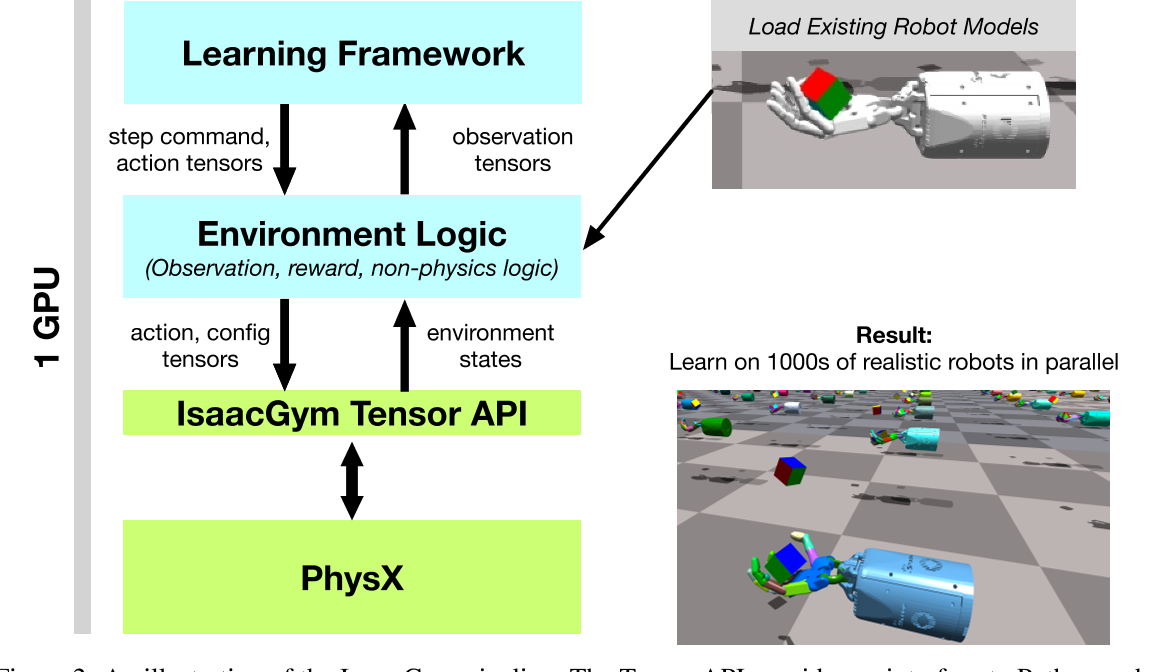
\includegraphics[width=0.8\linewidth]{isaac_workflow.png}
  
\end{figure}

图\ref{fig:isaac_workflow}展示了整个\emph{Isaac Gym}系统的工作架构,\emph{Isaac Gym}提供了一个直接API,用于创建和填充带有机器人和对象的场景,支持常见的\emph{URDF}和\emph{MJCF}文件格式来加载数据。每个环境可以根据需要重复多次,同时保留副本之间变化的能力(例如通过域随机化\cite[p]{Tobin_Fong_Ray_Schneider_Zaremba_Abbeel_2017})。各个环境同时模拟,与其它环境互不影响。\emph{Isaac Gym}还包括基本的近端策略优化 (PPO) 实现和一个简单的RL任务系统,但用户可以根据需要替代任务系统或RL算法。
\subsection[在Isaac上建立仿真]{在Isaac上建立仿真}

\subsection[张量API]{张量API}
\begin{figure}
  \centering
  \caption[View of tensors.]{View of tensorsIsaac\cite[p8]{Makoviychuk_Wawrzyniak_Guo_Lu_Storey_Macklin_Hoeller_Rudin_Allshire_Handa_et_al_2021}.}
  \label{fig:isaac_tensors_api}
  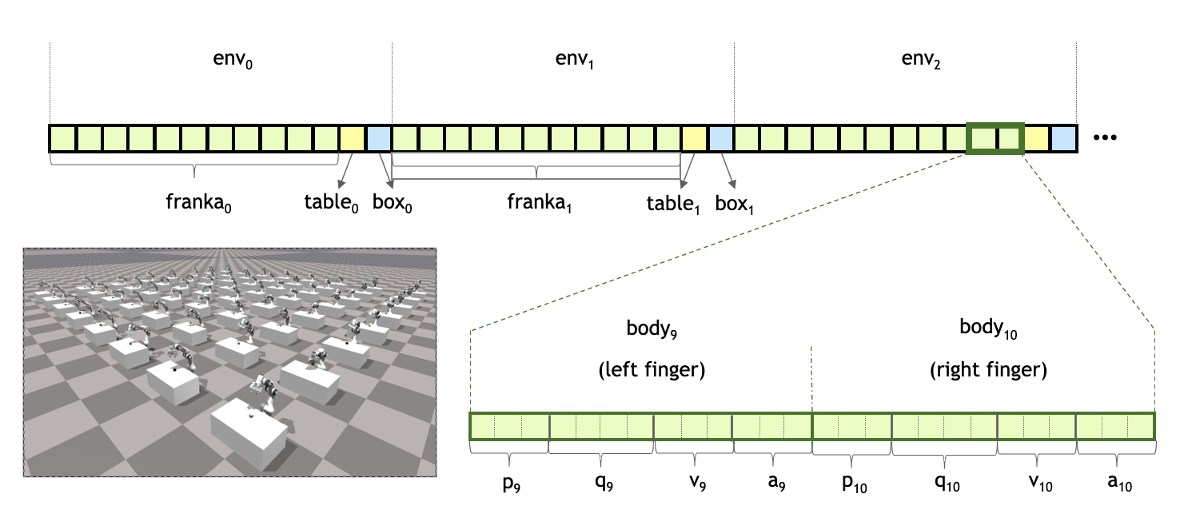
\includegraphics[width=1.0\linewidth]{isaac_tensors_api.png}
\end{figure}

\emph{Isaac Gym}在物理引擎上提供数据抽象层。这允许我们使用共享的前端API支持多个物理引擎,不仅限于\emph{PhysX}。

用户不是直接调用物理引擎函数,而是可以访问平面缓冲区中的所有物理数据。这种面向数据的方法使我们能够消除许多开销,这是由于在用户代码中循环超过数万个单个模拟参与者造成的。物理状态暴露于Python用户作为全局张量。例如,所有刚体状态都可以在单个刚体状态张量中找到。图\ref{fig:isaac_tensors_api}显示了一个典型的\emph{Isaac Gym}场景,由相同环境的各种副本组成,模拟并行运行的不同变体以及与它相关的相应张量。控制输入也可以使用全局张量应用。例如,将力应用于模拟中的所有刚体可以使用单个函数调用来完成,该函数调用取包含所有力的张量。用户可以创建全局张量的自定义视图或切片以适应他们的需求。当将多个环境实例打包到模拟中时,可以使用环境索引作为维度之一来创建数据的自定义视图。通过在多个环境中并行运行GPU内核,这使得向量化观察和奖励计算变得容易。


\subsubsection[Python接口]{Python接口}
\emph{Isaac Gym}的核心是使用\emph{C++}和\emph{CUDA}实现的。它完全独立于机器学习中常用的任何 Python框架。为了使Python用户可以轻松访问数据,\emph{Isaac Gym}提供实用程序,可以将原始数据缓冲区“包装”为PyTorch等常见机器学习框架中的张量对象。张量包装实用程序使得在没有任何复制开销的情况下使用Python共享本地CPU或GPU缓冲区成为可能。\emph{Isaac Gym}的一个强大功能是通过简单地打乱标志在CPU或GPU上运行相同代码的能力。Python用户不需要编写自定义\emph{C++}或\emph{CUDA}内核来计算观察、奖励或动作。当物理状态和控制张量被包装为\emph{PyTorch张量}时,用户可以利用\emph{TorchScript JIT}将他们的Python函数编译为低级脚本,可以快速编排训练管道。

\subsubsection[物理状态张量]{物理状态张量\label{section:physics_state_tensors}}
物理状态张量用于获得运行模拟的状态快照。Isaac Gym允许使用最大和最小坐标与模拟交互。物理状态包括刚体的运动学状态和自由度(DOF)。刚体状态由位置、方向(四元数)、线速度和角速度组成。自由度状态包括位置和速度。在下面的代码片段展示了如何通过 API 访问它们。

转动自由度使用弧度为单位,直线自由度使用米作为单位。其它提供的状态数据包括接触力、刚体力传感器和自由度力传感器。为了支持操作空间控制和逆运动学应用,\emph{Isaac Gym}还提供了可用于关节行为体的\emph{雅可比矩阵(Jacobian Matrix)}和\emph{广义质量矩阵(Mass Matrix)}。可用的状态张量列在表\ref{tb:physics_state_tensors}中
% \textcolor{red}{table to be added ...}

\begin{table}
  \centering
  \begin{threeparttable}[c]
    \caption[Physics state tensors.]{Physics state tensors. $N_A$ is the total number of actors, $N_B$ is the total number of rigid bodies (including articulation links), $N_D$ is the total number of degrees of freedom, and $N_F$ is the total number of rigid body force sensors.}
    \label{tb:physics_state_tensors}
    \begin{tabular}{L{2cm} L{6cm} L{2cm} L{2cm}}
      \toprule 
      Tensor & Description & Shape & Usage \\
      \midrule 
      Actor root state & State of all actor root bodies (position, orientation, linear and angular velocity). & ($N_A, 13$) & Get/Set\\ \midrule
      DOF state & State of all degrees of freedom (position, velocity). & ($N_D, 2$) & Get/Set\\ \midrule
      Rigid body state & State of rigid bodies (position, orientation, linear and angular velocity). & ($N_B, 13$) & Get\\ \midrule 
      DOF forces & Net forces experienced at each degree of freedom. & $N_D$ & Get\\ \midrule 
      Rigid body forces & Rigid body forces and torques experienced at force sensor locations. & ($N_F, 6$) & Get\\ \midrule 
      Net contact forces & Net forces experienced by each rigid body. & ($N_B, 3$) & Get\\ \midrule 
      Jacobian matrix & Jacobian matrices for a homogeneous group of actors. & Variable & Get\\ \midrule 
      Mass matrix & Generalized mass matrices for a homogeneous group of actors. & Variable & Get\\
      \bottomrule
    \end{tabular}
  \end{threeparttable}
\end{table}

% \textcolor{red}{code to be added ...}

\subsubsection[物理控制张量]{物理控制张量\label{section:physics_control_tensors}}
物理模拟输入包括力、力矩和PD控制,如位置和速度目标。力和力矩可以应用于刚体和自由度。PD目标应用于配置为使用位置或速度驱动器的自由度。用户可以使用单独的 API 配置刚度和阻尼等驱动参数。表\ref{tb:physics_control_tensors}列出了可用的控制张量。控制张量通常在 PyTorch 等更高级别的框架中创建,但可以使用张量包装实用程序与 Isaac Gym 有效地共享。

% \textcolor{red}{table to be added ...}

\begin{table}
  \centering
  \begin{threeparttable}[c]
    \caption[Physics control tensors.]{Physics control tensors. $N_B$ is the total number of rigid bodies (including articulation links), $N_D$ is the total number of degrees of freedom.}
    \label{tb:physics_control_tensors}
    \begin{tabular}{L{2cm} L{4cm} L{2cm} L{4cm}}
      \toprule 
      Tensor & Description & Shape & Applied to \\
      \midrule 
      DOF actuation forces & Torques or linear forces to be applied to degrees of freedom. & $N_D$ & All actors or indexed subset\\ \midrule
      DOF position targets & PD position targets for degrees of freedom. & $N_D$ & All actors or indexed subset\\ \midrule 
      DOF velocity targets & PD velocity targets for all degrees  of freedom. & $N_D$ & All actors or indexed subset\\ \midrule 
      Rigid body forces & Forces to be applied to rigid bodies. & ($N_B, 6$) & All rigid bodies\\ \midrule 
      Rigid body torques & Torques to be applied to rigid bodies. & ($N_B, 3$) & All rigid bodies\\ 
      \bottomrule
    \end{tabular}
  \end{threeparttable}
\end{table}

\begin{note}
  关于如何使用Python接口访问和获取这些\emph{物理状态张量(表\ref{tb:physics_state_tensors})}和\emph{物理控制张量(表\ref{tb:physics_control_tensors})}将在下面的章节中介绍。
\end{note}

\section[物理模拟器]{物理模拟器}

\begin{table}
  \centering
  \begin{threeparttable}[c]
    \caption[Simulator tuning parameters]{Parameters exposed to users to tune the simulator.}
    \label{tb:simulator_tune_parameters}
    \begin{tabular}{C{4cm} C{10cm}}
      \toprule 
      Parameter & Description\\
      \midrule 
      Delta time (dt) & Control time-step size\\
      Gravity & Control the gravity in the scene\\
      Collision filtering & Filters Collisions between shapes\\
      Position iteration & Biased (velocity + position error correcting) solver iterations\\
      Velocity iterations & Unbiased (velocity error only correcting) solver iterations\\
      Max bias coefficient & Limits the magnitude of position error bias Friction\\
      Restitution & Controls bounce\\
      Static/dynamic friction & Static and dynamic friction coefficients\\ \midrule 
      Bounce threshold & Relative normal velocity limit below which restitution is ignored\\ \midrule 
      Rest offset & Distance at which shapes are held separated. Default is 0 but can be increased to hold objects at gap. Useful for thin objects.\\ \midrule 
      Friction offset threshold & Distance at which shapes are held separated. Default is 0 but can be increased to hold objects at gap. Useful for thin objects.\\ \midrule 
      Friction offset threshold & Distance at which friction anchors are discarded (static friction depends on friction anchor caching)\\ \midrule 
      Solver offset slop & An epsilon value used to correct for round-off errors in contact gen. Corrects small skew effects with rolling spheres or capsules.\\ \midrule 
      Friction correlation distance & Distance at which contacts are merged into a single friction constraint\\ \midrule 
      Max force & Per-body and per-contact force limits\\
      Drive stiffness & Positional error correction coefficient of a PD controller\\
      Drive damping & Velocity error correction coefficient of a PD controller\\
      Joint friction Per-joint friction term. Simulates dry friction in a joint.\\
      Joint armature & Per-joint armature term - simulates motor inertia.\\
      Body/link Damping & World-space linear/angular damping on each body/link\\
      Max velocity & Linear/angular limit per-body\\
      \bottomrule
    \end{tabular}
  \end{threeparttable}
\end{table}

机器人模拟使用减少坐标关节的物理引擎\href{https://developer.nvidia.com/physx-sdk}{PhysX}。任何单个刚体都可以用最大坐标刚体或单连杆简化坐标关节来模拟。具有单连杆的关节和刚体的是等效的和可互换的。表\ref{tb:simulator_tune_parameters}描述了向用户公开的用于调优模拟器的各种参数。














% \section[PyTorch的使用]{PyTorch的使用}
% \textcolor{red}{\small
% 这部分结合Pytorch的官方文档和legge\_gym库提取其中关于\emph{.pth}模型的构建和使用流程和实例...
% }